\chapter{Materials and Methodology}
\section{Algorithms}
\subsection{Generative Adversarial Network}
Generative adversarial networks (GANs) are a class of artificial intelligence algorithms used in unsupervised machine learning, implemented by a system of two neural networks contesting with each other in a zero-sum game framework. They were introduced by Ian Goodfellow et al. in 2014. This technique can generate photographs that look at least superficially authentic to human observers, having many realistic characteristics.

The generative model is pitted against an adversary: a
discriminative model that learns to determine whether a sample is from the model distribution or the
data distribution. The generative model can be thought of as analogous to a team of counterfeiters,
trying to produce fake currency and use it without detection, while the discriminative model is
analogous to the police, trying to detect the counterfeit currency. Competition in this game drives
both teams to improve their methods until the counterfeits are indistiguishable from the genuine
articles.

The discriminator network is a standard convolutional network that can categorize the images fed to it, a binomial classifier labeling images as real or fake. The generator is an inverse convolutional network, in a sense: While a standard convolutional classifier takes an image and downsamples it to produce a probability, the generator takes a vector of random noise and upsamples it to an image. The first throws away data through downsampling techniques like maxpooling, and the second generates new data as shown.


\begin{figure}
 \centering
 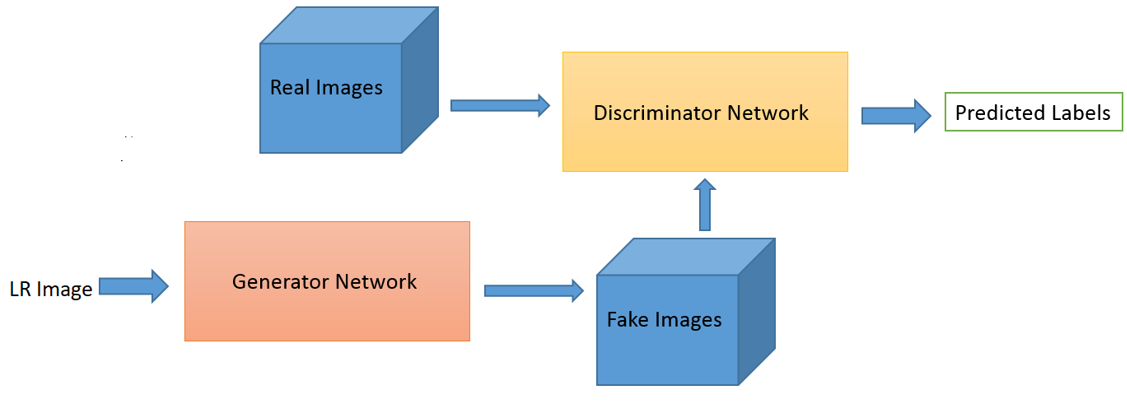
\includegraphics[scale=0.5]{gan_model}
 \caption{GAN workflow diagram}
 \label{fig:ganmodel}
\end{figure}

The entire process can be summerized as a game theoretic framework where two player D and G play the following two-player minimax game with value function V(G,D):
\begin{equation}
\min_{G}\max_{D}V(D,G) = E_{x\sim p_{data}(x)}[log D(x)] + E_{z\sim p_z(z)}[log( 1 - D(G(z)))] 
\end{equation}
The essence of the equation is that the generator tries to decrease the entropy of the system while the discriminator  tries to increase the entropy of the system.Decreasing the entropy of the system allows to increase the predictability of the system.Hence the generator becoming more accurate.

The steps taken by the GAN are: 
\begin{itemize}
 \item The generator takes in low-resolution image  and returns a high-resolution-image
 \item This generated image is fed into the discriminator alongside a stream of high-resolution images taken from the actual dataset.
 \item The discriminator takes in both real and fake images and returns probabilities, a number between 0 and 1, with 1 representing a prediction of authenticity and 0 representing fake.
\end{itemize}
\begin{algorithm}[H]
\DontPrintSemicolon
\For{number of training iterations}{
 \For{k steps do}{
   Sample minibatch of m low-resolution images $ \{z^1,\dots,z^m\}$ from prior $p_g(z)$\;
   Sample minibatch of m examples of high resolution images $\{ x^1,\dots,x^m\}$ from data generating distribution $p_data(x)$\;
   Update the discriminator by ascending its stocastic gradient:\;
   \begin{equation}
     \nabla_{\theta_d} \frac{1}{m} \sum_{i=1}^{m}[log D(x^i) + log(1 - D(G(z^i)))]
    \end{equation}\;
  }
  Sample minibatch of m low resolution image samples $\{z^1 \dots z^m\}$ from prior $p_g(z)$\;
  Update the generator by descending its stochastic gradient:\;
  \begin{equation}
    \nabla_{\theta_g}\frac{1}{m}\sum_{i=1}^{m}log(1 - D(G(z^i)))
  \end{equation}\;
}
The gradient-based updates can use any standard gradient-based learning rule.We used adam-optimizer in our experiments.\;
\caption{Minibatch stochastic gradient descent training fro generative adversarial nets. The number of steps to apply to the discriminator ,k ,is a hyperparameter.}
\end{algorithm}
\subsection{Batch Normalization}
Training Deep Neural Networks is complicated by the fact that the distribution of each layer’s inputs changes during training, as the parameters of the previous layers change. This slows down the training by requiring lower learning rates and careful parameter initialization, and makes it notoriously hard to train models with saturating nonlinearities.  We refer to this phenomenon as internal covariate shift,  and  address the  problem by  normalizing layer inputs. It accomplishes  this  via  a  normalization  step  that  fixes  the
means and variances of layer inputs. Batch Normalization
also has a beneficial effect on the gradient flow through
the  network,  by  reducing  the  dependence  of  gradients
on the scale  of the parameters or of their initial values.
This  allows  us  to  use  much  higher  learning  rates  without the  risk  of  divergence

Consider a mini-batch B of size m. Since the normalization is applied to each activation independently, let us focus on a particular activation $x^{(k)}$ and omit k for clarity. We have m values of this activation in the mini-batch,
\begin{equation}
 B = \{x_{1 \dots m}\}
\end{equation}

Let the normalized values be $\hat{x_{1 \dots m }}$ , and their linear transformations  be $y_{1 \dots m}$. The BN Transform in Algorithm is shown below.

\begin{algorithm}[H]
\DontPrintSemicolon
\KwIn{Values of x over a mini-batch: B = \{ $x_{1 \dots m}$\}; Parameters to be learned: $\gamma ,\beta$ }
\KwOut{ \{ $y_i = BN_{\gamma,\beta}(x_i)$\}}
$\mu_B \leftarrow \frac{1}{m}\sum_{i=1}^{m}x_i$\tcp{mini-batch mean}
$\sigma_B^2 \leftarrow \frac{1}{m}\sum_{i=1}^{m}(x_i - \mu_B)^2$  \tcp{mini-batch variance}
$\hat x_i \leftarrow \frac{x_i - \mu_B}{\sqrt{\sigma_B^2 + \epsilon}}$  \tcp{normalize}
$y_i \leftarrow \gamma\hat x_i + \beta \equiv BN_{\gamma,\beta}(x_i) $  \tcp{scale and shift}
\caption{Batch Normalization Transform applied to activation x over a mini-batch}
\label{algo:batchnorm}
\end{algorithm}
The algorithm used in Algorithm \ref{algo:batchnorm} can be extended to normalize the entire activations rather than a single activation function.
Thereby normalizing the entire network with the additional learning parameters $\beta$ and $\gamma$.

\begin{algorithm}[H]
\DontPrintSemicolon
\KwIn{Network N with trainable parameters $\theta$ ; subset of activations $\{ x^{(k)}\}_{k=1}^K$}
\KwOut{Batch-Normalized network for inference, $N_{BN}^{inf}$}
$N_{BN}^{tr} \leftarrow N$ \tcp{Training BN network}
\For{ $k = 1\dots K$}{
 Add transformation $y^{(k)} = BN_{\gamma^{(k)},\beta^{(k)}}{(x^{(k)})}$ to $N_{BN}^{tr}$ (Alg \ref{algo:batchnorm})\;
 Modify each layer in $N_{BN}^{tr}$ with input $x^{(k)}$ to take $y^{(k)}$ instead\;
}
Train $N_{BN}^{tr}$ to optimize the parameters $\theta \cup \{ \gamma^{(k)} ,\beta^{(k)} \}_{k=1}^K$\;
$N_{BN}^{inf} \leftarrow N_{BN}^{tr}$ \tcp{Inference BN network with frozen parameters}
For{ $k = 1 \dots K$}{
 \tcp{For clarity $x \equiv x^{(k)} , \gamma \equiv \gamma^{(k)} , \mu_B \equiv \mu_B^{(k)}$}
 Process muliple training mini-batches $B$, each of size $m$, and average over them:
 \begin{equation}
   E[x] \leftarrow E_B[\mu_B]
 \end{equation}
 \begin{equation}
   Var[x] \leftarrow \frac{m}{m-1} E_B[\sigma_B^2]
 \end{equation}\;
 In $N_{BN}^{inf}$, replace the transform $y = BN_{\gamma,\beta}{(x)}$ with 
 \begin{equation}
  y =  \frac{\gamma}{\sqrt{Var[x] + \epsilon}} x (\gamma - \frac{\gamma E[x]}{\sqrt{Var[x] + \epsilon}})
 \end{equation}
}
\caption{Training a Batch-Normalized Network}
\label{algo:batchnorm2}
\end{algorithm} 
\subsection{Pixel Shuffler}
The previous works on image super-resolution using deep learning  where based on initally interpolating the low-resolution image $\textbf{I}_{LR}$ to high-resolution image by means of bicubic interpolation and the interpolated image is fed as input into the network for extracting features.Thinking from first principles, if it where possible to give the low resolution image as input the network could have learned more features within the same complexity as learning less features with the bicubically high-resolved image.
\begin{figure}[h!]
 \centering
 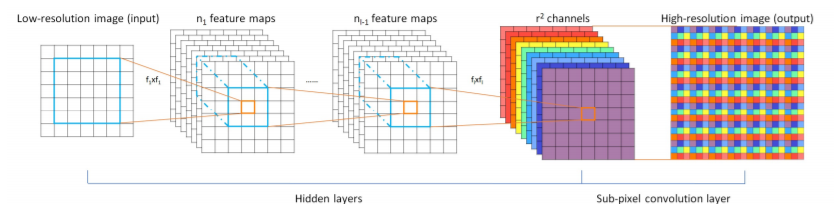
\includegraphics[scale=0.5]{pixel_shuffler}
 \caption{Pixel shuffler operation}
 \label{fig:pixelshuffler}
\end{figure}

The Pixel shuffler allows to reshape the input tensor of size $ H \times W \times Cr^2 $into that of size $rH \times rW \times C$ using the below equation
\begin{equation}
\textbf{I}^{SR} = f^L(\textbf{I}^{LR}) = PS(W_L * f^{L-1}(\textbf{I}^{LR}) + b_L)
\end{equation}
where f is the activation function used in each layer and $W_L$ is the kernal applied on the last layer L, * represents the convolution operator and  PS is a periodic suffling operator that does the rearrangement described as
\begin{equation}
PS(T)_{x,y,c} = T_{\floor{\frac{x}{r}},\floor{\frac{y}{r}},C*r*mod(y,r) + C*mod(x,r)+c}
\end{equation}
where x,y,c are the co-ordinates of the upscaled image.
\subsection{Graphics Processing Unit}
For this project two diffrent Graphics Processing Units where used \textbf{NVIDIA Jetson TX1} and \textbf{NVIDIA QUADRO M5000}.The computational power of each device helped to advance in training the generative models in much faster pace by exploiting the fast tensor calculation mechanisms employed on the system.

\subsubsection{NVIDIA JETSON TX1}
This AI supercomputer features NVIDIA Maxwell architecture, 256 NVIDIA CUDA cores, 64-bit CPUs, and a power-efficient design. Plus, it includes the latest technology for deep learning, computer vision, GPU computing, and graphics—making it ideal for embedded AI computing.It comes with 4GB ram of memory and 16GB eMMC external memory.
\begin{figure}[h!]
 \centering
 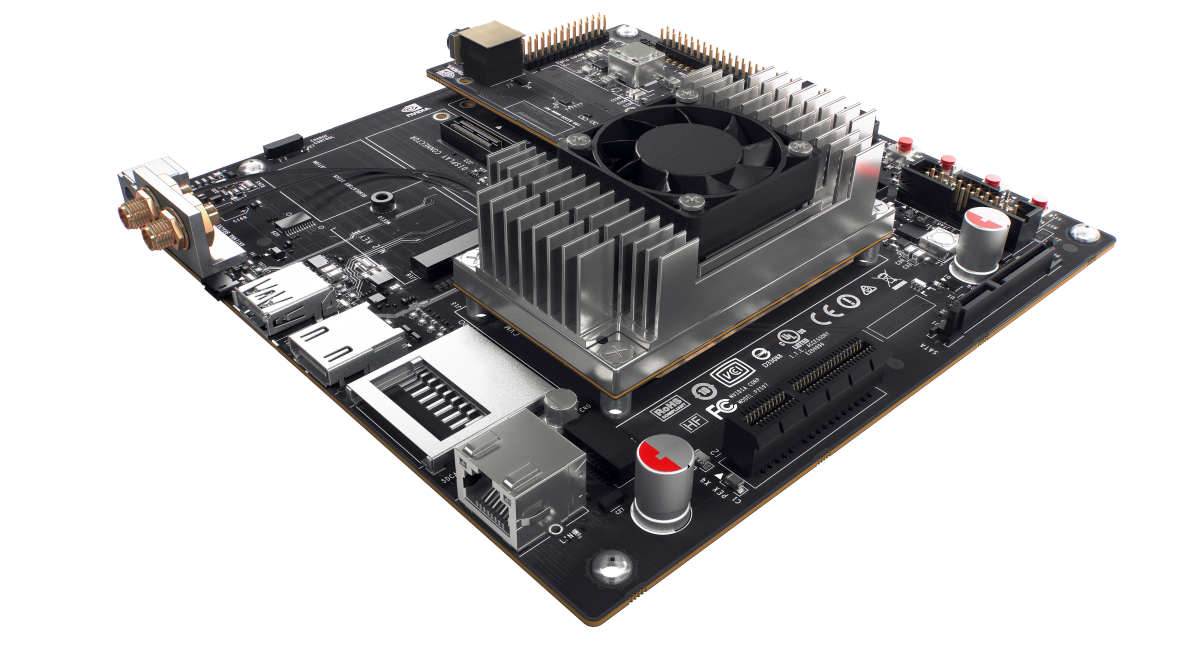
\includegraphics[scale=0.25]{jetsontx1}
 \caption{NVIDIA JETSON TX1}
 \label{fig:jetson}
\end{figure}
\subsubsection{NVIDIA QUADRO M5000}
Nvidia Quadro M5000 designed for extreme performance and power efficiency. Get real interactive expression with Nvidia Quadro the world’s most powerful workstation graphics. Nvidia’s advanced maxwell GPU architecture delivers incredible performance to let you unleash your creativity and conquer extreme workloads with ease. 8 GB of ultra-fast memory with ECC lets you create and render large, complex models and compute massive datasets.
\begin{figure}[h!]
 \centering
 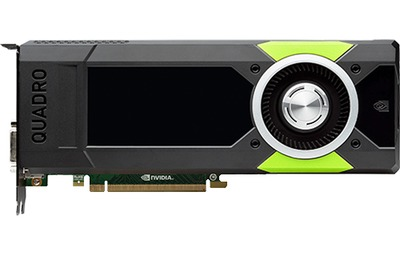
\includegraphics[scale=0.5]{quadrom5000}
 \caption{NVIDIA QUADRO M5000}
 \label{fig:quadro}
\end{figure}